
\subsection{What is \LaTeX?}
LaTeX (pronounced \enquote{Lah-Tech}) is a document preparation system for technical and scientific documents. LaTeX is not a word processor; instead, the system encourages authors to focus on content rather than the appearance of their documents\footnote{\url{https://www.latex-project.org/about/}}. 

\begin{minipage}{\linewidth}
\fbox{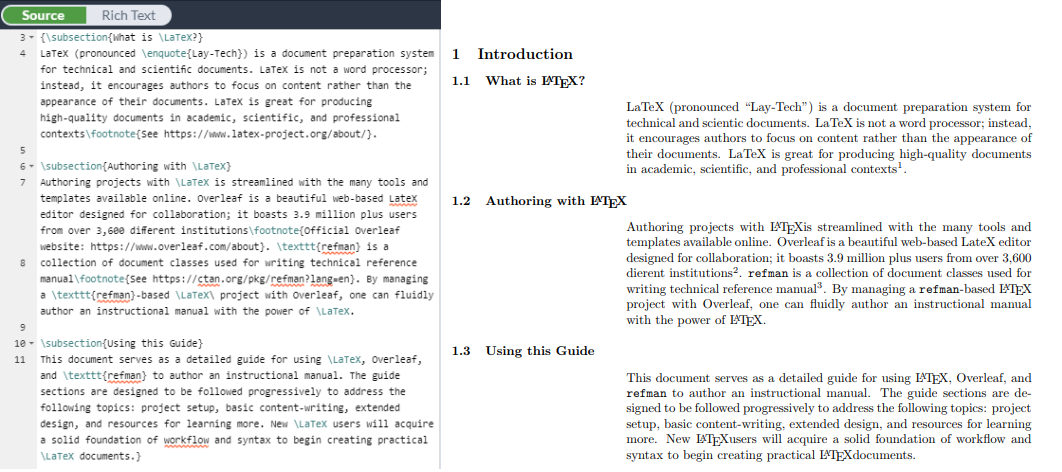
\includegraphics[width=\linewidth]{graphics/IntroSource.png}}
\captionof{figure}{\LaTeX\ document example}
\end{minipage}

By delegating document formatting to templates and focusing on content, \LaTeX\ authors can efficiently produce large technical documents that look great. Individuals can reuse templates and projects for consistent style across a large organization.
\par
\LaTeX\ is suitable for producing high-quality technical documents in both academic and professional contexts.

\subsection{Authoring with \LaTeX}
Authoring projects with \LaTeX\ is streamlined with the many tools and templates available online.
\par
Overleaf is a beautiful web-based \LaTeX editor designed for collaboration; it boasts 3.9 million plus users from over 3,600 different institutions\footnote{\url{https://www.overleaf.com/about}}.
The software has many powerful features including Git integration, change tracking, and rich text editing\footnote{\url{https://www.overleaf.com/blog/overleaf-v2-launch-announcement}}.

\begin{minipage}{\linewidth}
\fbox{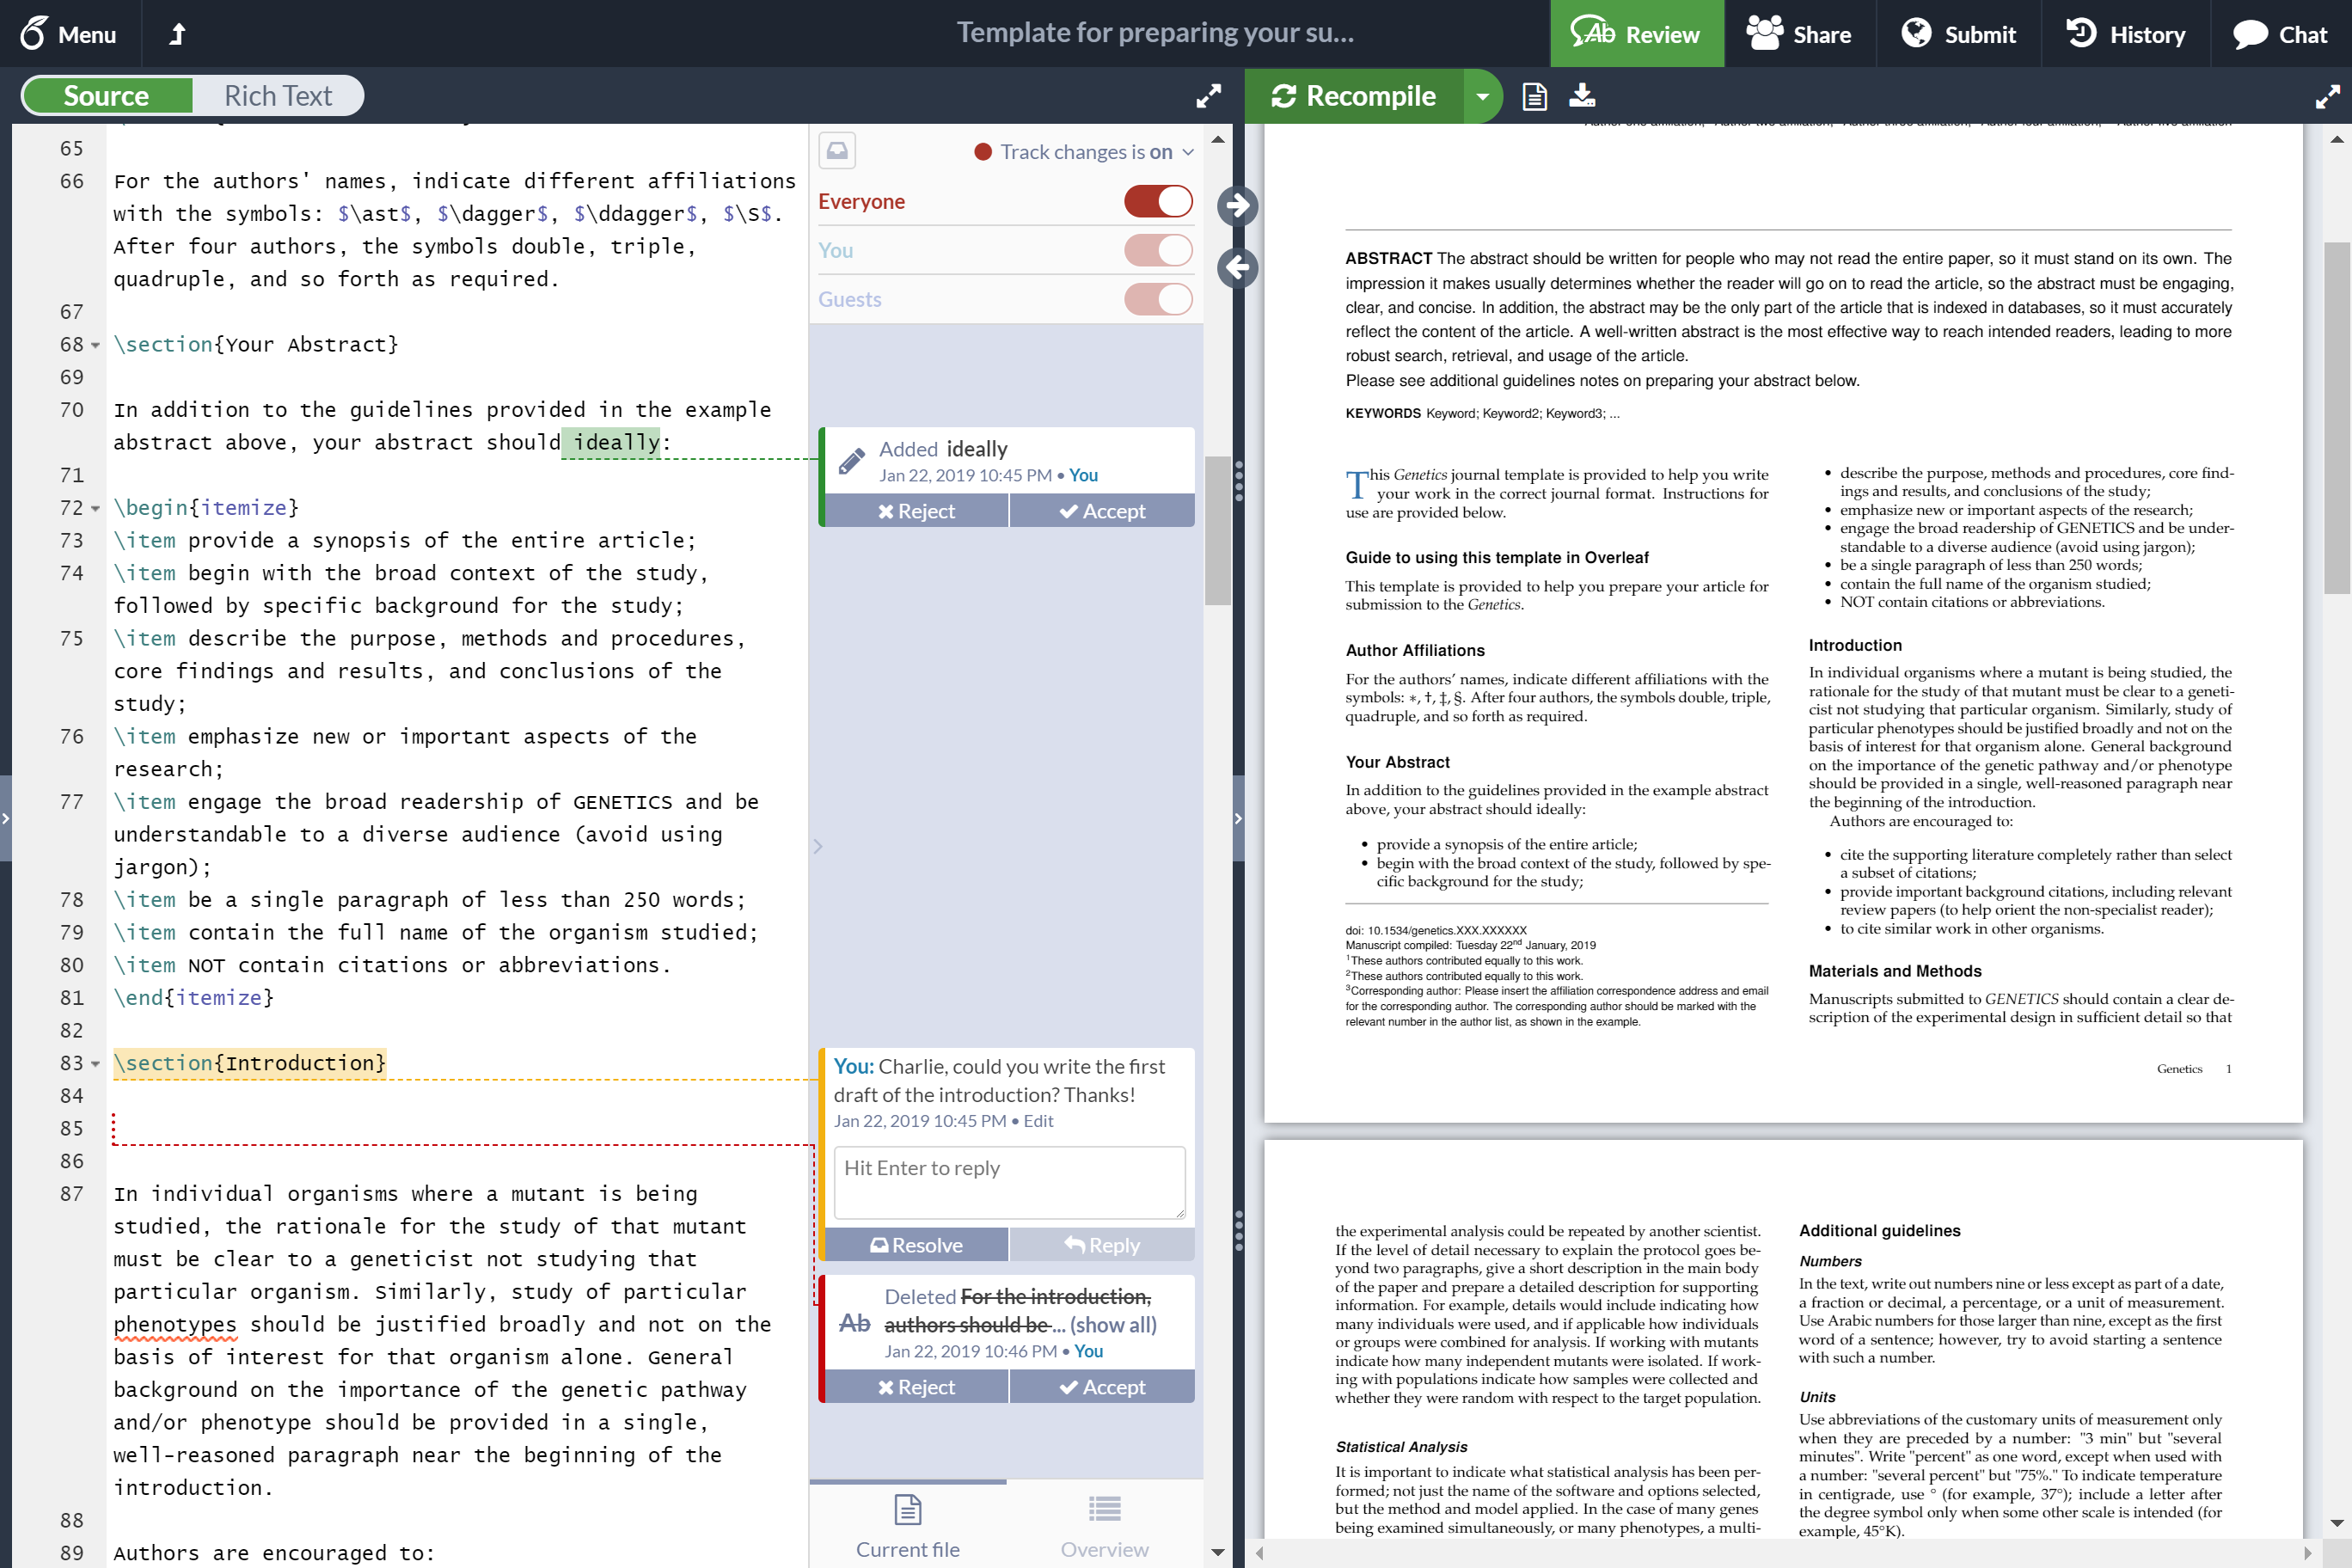
\includegraphics[width=\linewidth]{graphics/OverleafProduct.png}}
\captionof{figure}{Feature demonstration of Overleaf}
%https://www.overleaf.com/for/press/resources
\end{minipage}

\texttt{refman} is a collection of document classes used for writing technical reference manuals\footnote{\url{https://ctan.org/pkg/refman?lang=en}}; it includes formatted structure for document title page, table of contents, sections, and more. As a template, \texttt{refman} provides a polished starting point for technical reference manuals and guides.

\begin{minipage}{\linewidth}
\fbox{
\includegraphics[width=\linewidth]{graphics/refman.PNG}}
\captionof{figure}{Title page of compiled \texttt{refman}}
%http://ctan.math.illinois.edu/macros/latex/contrib/refman/layout_e.pdf
\end{minipage}

By using Overleaf and \texttt{refman}, authors can quickly create formatted instructional guides with the power of \LaTeX.

\subsection{Using this Guide}
This document serves as an instructional guide for using \LaTeX, Overleaf, and \texttt{refman} to author a technical document; it covers more than just \LaTeX\ syntax. Overleaf setup, \texttt{refman} template importing, and project organization are also explained to provide readers with a practical grasp of the \LaTeX\ document preparation process. 
\par
Unlike other guides, this one focuses on practical minimums for creating a document with \LaTeX. Beginner \LaTeX\ users are encouraged to take advantage of existing resources to streamline use and learning of \LaTeX. Though this guide is designed to be followed step-by-step, specific tasks from individual sections can be applied at any point after project setup
\par
 After learning about workflow, syntax, and basic commands, new \LaTeX\ users will be able to create practical \LaTeX\ guides. Informational resources and links are included at the end of this guide for further learning. Curiosity and desire to improve drives the development of \LaTeX\footnote{\url{https://lamport.azurewebsites.net/pubs/lamport-latex-interview.pdf}}; in the same spirit, let it fuel the revolution of your document preparation process!
\par

